\section{Hazard}
\label{sec:hazard} 

\begin{figure}[ht]
    \centering
    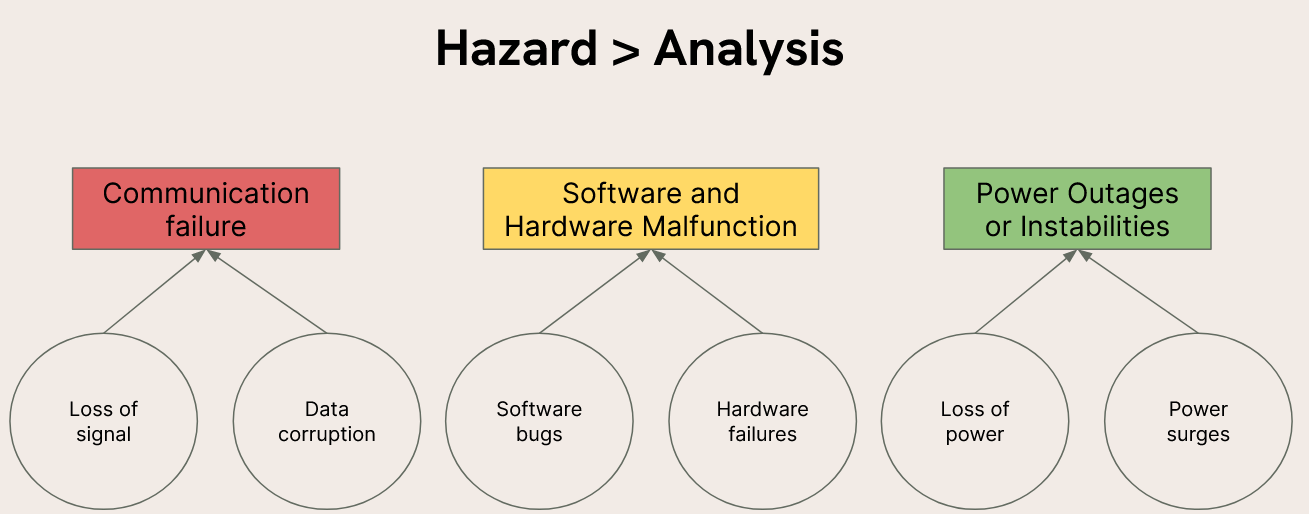
\includegraphics[width=0.5\textwidth]{images/hazard_analysis.png}
    \caption{Diagram outlining the main categories of hazards.}
    \label{fig:hazard_categories}
\end{figure}

The diagram is organized into three main categories of hazards. An overview of the hazards illustrated in Figure \ref{fig:hazard_categories}

\begin{enumerate}
    \item Communication Failure: This category identifies the risks associated with the failure of communication systems. Subcategories include:
    \begin{enumerate}
        \item Loss of Signal: This can mean interruption of communication lines or signals, which can lead to a lack of coordination or response in a critical situation.
        \item Data Corruption: This hazard involves the alteration of data during transmission, which may result in incorrect information and action.
    \end{enumerate}

    \item Software and Hardware Malfunction: This category refers to potential problems with software and hardware components of the system. Subcategories include:
    \begin{enumerate}
        \item Software Bugs: Flaws or errors in software code that can cause unexpected behavior or system failures.
        \item Hardware Failures: Physical malfunctions or breakdowns of hardware components that can cause system malfunctions or improper operations.
    \end{enumerate}

    \item Power Failures or Fluctuations: This category focuses on the power supply and the risks associated with its failures or fluctuations. Subcategories include:
    \begin{enumerate}
        \item Power Loss: Complete power failures that can shut down an entire system or individual critical components.
        \item Power Surges: Power surges that can damage equipment, corrupt data, or cause erratic system behavior.
    \end{enumerate}
\end{enumerate}

\begin{figure}[ht]
    \centering
    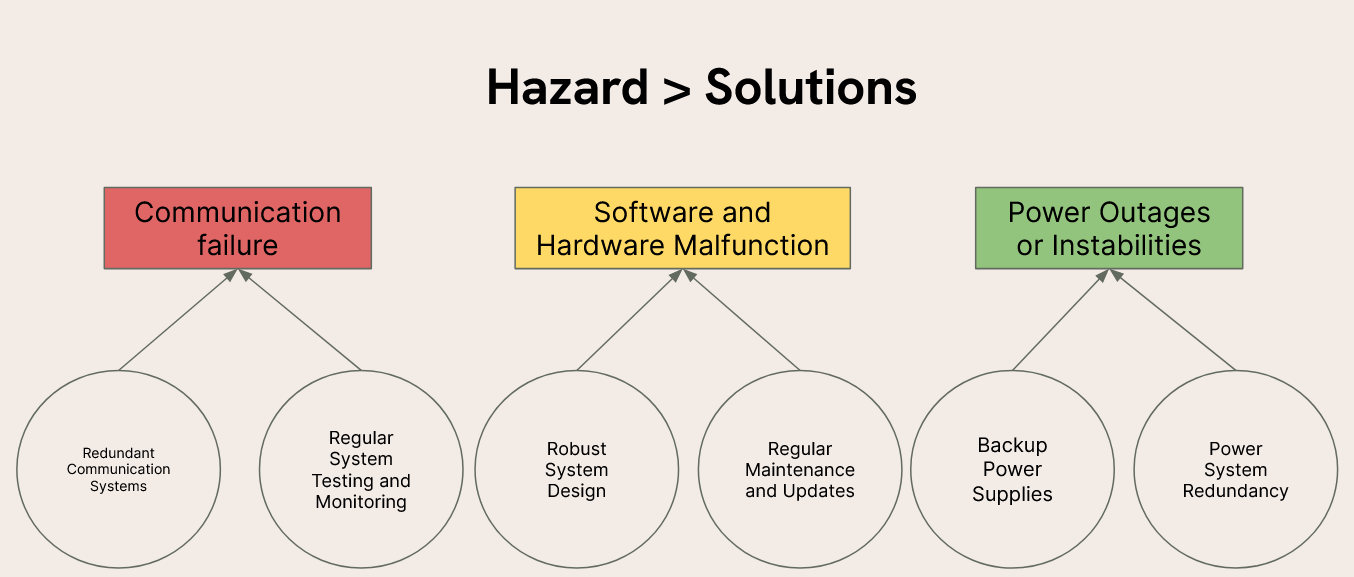
\includegraphics[width=0.5\textwidth]{images/hazard_solutions.png}
    \caption{Solutions to address the identified hazards.}
    \label{fig:hazard_solutions}
\end{figure}

Solutions illustrated in Figure \ref{fig:hazard_solutions}.Solutions to address these hazards include:

\begin{enumerate}
    \item Solutions to Address Communication Failures:
    \begin{enumerate}
        \item Redundant Communication Systems: Implementing redundant systems ensures continuous and reliable communication by having backup channels or methods that can take over in case the primary communication path fails.
        \item Regular System Testing and Monitoring: Regular testing and monitoring of communication systems help detect and correct faults before they lead to failure, thus preventing signal loss or data corruption.
    \end{enumerate}

    \item Solutions for Software and Hardware Faults:
    \begin{enumerate}
        \item Robust System Design: A robust system design includes using high-quality components, developing fault tolerance, and implementing error-handling procedures to prevent complete system failure if a component fails.
        \item Regular Maintenance and Updates: Regular maintenance and software updates can address hardware problems and software bugs, preventing them from leading to failures.
    \end{enumerate}

    \item Solutions for Power Outages or Instabilities:
    \begin{enumerate}
        \item Backup Power Supplies: Backup power solutions, like Uninterruptible Power Supplies or generators, provide immediate power to ensure that critical components remain operational during outages.
        \item Power System Redundancy: Power system redundancy, involving alternative power sources or redundant power delivery paths, ensures the availability of power to critical system components at all times.
    \end{enumerate}
\end{enumerate}
